\chapter{Brief introduction to sciences using neutrons}
\chaptermark{Brief introduction to sciences using neutrons}
\cleardoublepage

\minitoc

\section{Introduction}
\begin{refsection}
  \label{ch1:Introduction}
  This chapter introduces the general context behind the European Spallation Source (ESS), which is a facility in construction in Lund (Sweden). As every spallation source, it will make use of a particle accelerator and a heavy metal target to create neutrons. Even if, the work presented in this thesis strictly concerns the accelerator part alone, it is important to give a quick overview of neutron science to answer the following question: "Why building a 1.8 \texteuro billion euros neutron source is crucial for science in Europe?"

  After a brief historical review about the neutron discovery, this chapter presents what a neutron is and why its properties are interesting for probing matter and structures. A concrete application of neutron science will be illustrated. Finally, the different ways of producing neutrons are also briefly presented as well as the advantages and drawbacks of each method.

  \section{History}
  Historically, the neutron was the last component of the atom to be discovered. The electron was discovered first by J.J. Thomson in 1897 using a vacuum tube. The electrons are elementary negatively charged components of all atoms. Since, the atoms are neutral there must be an other component of the atom with an opposite charge. However, Thomson was not able to really answer the question of how the atom is structured.

  Almost in parallel, the discovery of natural radioactivity by H. Becquerel in 1896 and M. and P. Curie in 1898 opened a new field of possibility for physical experiments. In 1909, E. Rutherford observed that atoms consist of nuclei that concentrate all mass and charges \cite{Rutherford:1911zz}.
  From this observation he proposed a new atomic model, later improved by N. Bohr. Then in 1919, he observed that light atoms eject hydrogen when they are impinged by alpha particles: the proton was discovered. However, this experiment does not explain the differences of mass and of charge between atoms.

  In 1930, W. Bothe and H. Becker found out that neutral radiations were emitted when beryllium, boron or lithium were bombarded by alpha particles (original paper \cite{Bothe1930}), but they were unable to understand, and actually misinterpreted, the nature of these neutral particles.

  By means of an ionization chamber, few years later, I. and F. Joliot-Curie observed that the neutral radiation, produced as described above, generated protons when it impacted on a light hydrogen-based compound. However, they concluded that the proton ejection could be due to a photon scattering (similar to Compton scattering which was discovered 8 years before) \cite{curie:jpa-00233129}.

  In 1932, J. Chadwick performed a more accurate measurements of proton recoils for several light elements \cite{Chadwick1932}. He discarded the hypothesis of an elastic collision with gamma rays on the basis of energy and momenta conservation. The neutral particle had to have a mass close to that of protons: the neutron was discovered.

  \section{Neutron and neutron interaction with matter}
  \label{ch1:sec:Neutron}
  A neutron is a non-elementary particle with no charge. Its mass is $939.56\,\mathrm{MeV/c^{2}}$ ($1.67 \cdot 10^{-27}\,\mathrm{kg}$). A neutron does not have the strong electromagnetic interaction with the electrons of atoms, unlike charged particles and photons. Neutrons can travel long distances without major interactions. The neutron has a spin of $\frac{1}{2}$ and a low magnetic moment. Therefore it is possible to polarize a neutron beam. The magnetic moment allows the interaction with magnetic fields in the structure of matter. A neutron interacts mainly with the elements of the nucleus through strong interactions. A free neutron has a lifetime of $881.5\,\mathrm{s}$ and decays into a proton, an electron, and an antineutrino.
  Following the principle of wave-particle duality, neutrons can be described both as particles and as waves. By exploiting the De Broglie equation, the energy $E_{n}$ and wavelength $\lambda$ associated to a neutron are related by:

  \begin{equation*}
    E_{n} = \frac{h^{2}}{2m_{n}\lambda^{2}}
  \end{equation*}

  It is convenient to classify neutrons on the basis of the two above mentioned observables as "relativistic", "fast", ... as shown in Table \ref{chap1:tab:neutronsT}.

  %Neutron can be classified in several domains with more or less arbitrary limits:
  \begin{table}[ht]
  \centering
  \caption[Neutron classification according to the neutron energy and wavelength]
  {Neutron classification according to the neutron energy and wavelength. Different sources report different conventions. The range  limits here presented are taken from \cite{psiNeutronRange}.}
  \label{chap1:tab:neutronsT}
  \begin{tabularx}{\linewidth}{lXXX}
    \toprule
    Characteristic        & Energy               & Speed                              & Wavelength                                    \\
    \midrule
    Fast neutrons         & $>1\,\mathrm{MeV}$   & $>1.38\cdot 10^{7}\,\mathrm{m/s}$  & $>2.86\cdot 10^{-4}\,\mathrm{\si{\angstrom}}$ \\
    Intermediate neutrons & $>1\,\mathrm{eV}$    & $>1.38 \cdot 10^{4}\,\mathrm{m/s}$ & $>0.28\,\mathrm{\si{\angstrom}}$              \\
    Epithermal neutrons   & $>100\,\mathrm{meV}$ & $>4.37 \cdot 10^{3}\,\mathrm{m/s}$ & $>0.9\,\mathrm{\si{\angstrom}}$               \\
    Thermal neutrons      & $>12\,\mathrm{meV}$   & $>1.51 \cdot 10^{3}\,\mathrm{m/s}$ & $>0.28\,\mathrm{\si{\angstrom}}$              \\
    Cold neutrons         & $>0.12\,\mathrm{meV}$ & $>151\,\mathrm{m/s}$               & $>26\mathrm{\si{\angstrom}}$                  \\
    Ultra cold neutrons   & $<300\,\mathrm{neV}$ & $<6\,\mathrm{m/s}$                 & $<500\,\mathrm{\si{\angstrom}}$               \\
    \bottomrule
  \end{tabularx}
\end{table}


  Fast neutrons can be slowed down to the desired energy with the help of moderators. These moderators are mainly composed of light elements. Indeed the energy transfer during elastic scattering on light elements is efficient. The most common moderators are hydrogen, water, heavy water and graphite.

  There are several processes behind the interaction of neutrons with matter \cite{Leo1994} that can be classified in two categories: collision or absorption processes.
  In a collision where the nucleus structure remains the same. The collision can be:
  \begin{itemize}
    \item Elastic: in a (n,n) collision the kinetic energy of the system is preserved. The neutron can transfer part of its kinetic energy to the nucleus. If so, the direction of the neutron is changed.
    \item Inelastic: in (n,n') collision the kinetic energy of the system is not preserved and therefore the target nucleus is left in an excited state.
  \end{itemize}
  In absorption processes, the nucleus structure is altered by the neutron.
  Such processes can be subdivided as follows:
  \begin{itemize}
    \item Radiative capture: in (n,$\gamma$) reactions, the neutron is captured by the nucleus followed gamma emission
    \item Particle emission: in (n,p), (n,$\alpha$), ... but also (n,2n), (n,np),... reactions, the compound nucleus ejects one or more nucleons, or even a cluster of nucleons
    \item Fission: this phenomenon concerns heavy elements which, under the impact of a neutron, separate into (most of the times) two lighter elements
  \end{itemize}

  The above listed processes occur for incident neutron energies up to hundreds of MeV. The total neutron cross section (reaction probability) for a certain isotope, is the sum of all previous interaction cross sections.

  Above few hundreds MeV (pion production threshold) more interactions take place. The measurements of neutron cross sections remain a fundamental aspect of nuclear physics and application.

  % These three absorption processes occur mainly when the neutron energy is low. There are also other high-energy absorption phenomena. The total cross section is the sum of all previous cross sections, which leads to quite complex cross section spectra. 

  \section{Application of neutron probes}
  % TODO: Reférence
  Soon after neutron discovery in 1932, neutron scattering was found to be a unique tool for probing matter.  The use of advanced neutron scattering methods for investigating different materials became really popular in the 1960s, with the rise of research reactors. Since, as seen in the previous paragraph, different neutron energies correspond to different wavelengths, neutrons of diverse speeds can access diverse type of information. The energy selection influences also the selection of the field of application:  nuclear science or engineering. More techniques based on neutron scattering have been developed, each one relying on the peculiar characteristics of the incident neutral nucleons. In the present section, the different techniques are introduced in simplified manner to illustrate the huge possibilities provided by neutron scattering. A more rigorous approach can be found on the websites of the various institute specialized in this domain \cite{LLBinfo,ILLinfo,ISISinfo}.

  Neutron radiography is an imaging method that measures the transmission of neutrons in a sample. This method is similar to the well-known X-ray radiography. However, neutrons are more sensitive to light elements whereas for X-rays the higher the atomic number of the material they pass through, the more efficient is their attenuation. Neutrons have the ability to probe structure deeply and give good contrasts on dense materials. Neutron radiography is therefore an interesting complement to the X-rays one and these two methods are often combined. Its applications are extremely varied: from explosives imaging to archaeology. For instance, Fig. \ref{chap1:fig:Dague} shows a comparison between  X-ray and neutron radiography performed on an Indonesian dagger sheath. One can see that the neutrons give a good information of the internal wooden structure whereas the X-rays allow a fine detail of the metallic surface of the sheath.

  Reflectometry is mainly used to characterize the surface of samples such as thin films, interfaces and layered structures. In reflectometry, a monochromatic neutron beam is projected on the surface of the sample to be tested. The reflection profile is measured as a function of the incidence angle and neutron energy.

  Diffraction is a wide family of techniques for studying the diffraction pattern of a sample subjected to a neutron flux. The scale of measurement is in the order of nanometer to below {\AA}ngström range. This technique is mainly used to study the properties of crystals and powders.

  \begin{figure}[!ht]
	\begin{center}
		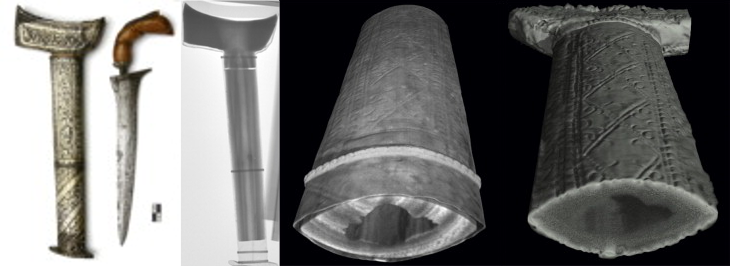
\includegraphics[width=\textwidth]{01_Introduction/figures/fig000_Dague}
	\end{center}
	\caption[]{\cite{LEHMANN2012S35}}
	\label{chap1:fig:Time_Scale}
\end{figure}


  The Small Angle Neutron scattering (\acrshort{sans}) is a specific diffractive and reflective techniques and is used to probe nanostructures. The method is very interesting for studying molecules, polymers, drugs... The typical setup of a SANS experiment is as follows: a collimated neutron beam, selected in speed with a monochromator, is sent directly to the sample. Some of the incident neutrons are deflected due to elastic collisions. The angle between the deflected neutrons and the beam is measured by mean of a 2D detector located several meters further along the beam axis.

  The latest technique is neutron spectrometry which consists in measuring the energy of the neutrons after an inelastic scattering on the sample. Several setup are possible to characterize scattered neutrons: Time of Flight (ToF) measurement, triple-axis method, spin echo measurement and backscattering spectrometry. Each of these detections covers different spatial and temporal ranges. For instance, ToF measurements are particularly suitable for short timescale whereas spin echo methods have very good resolutions at low neutron energies.

  All the methods presented above can be combined together to perform more advanced measurements. Fig. \ref{chap1:fig:Time_Scale} shows the different methods using neutrons with the scale of the different time and wavelength magnitudes. To take advantage of these methods it is necessary to have access to a neutron source, and to be concise, the brighter the source, the more efficient (in terms of statistics acquired in a certain time and therefore accuracy) the measurement.

  \begin{figure}[!ht]
	\begin{center}
		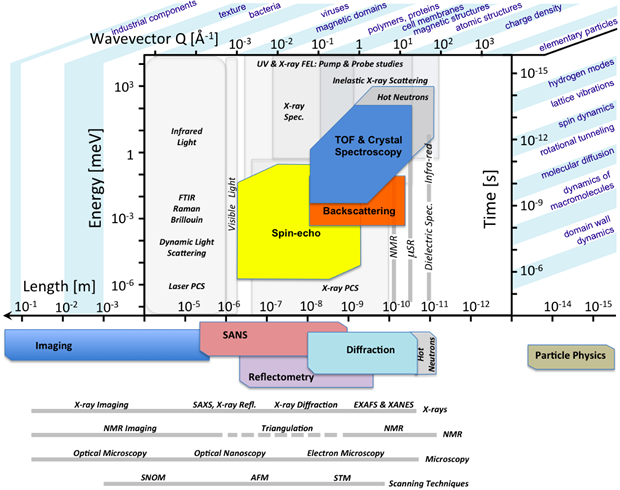
\includegraphics[width=\textwidth]{01_Introduction/figures/fig000_Time_Scale}
	\end{center}
	\caption[Ranges of distances and times of existing neutron scattering techniques]{Ranges of distances and times of existing neutron scattering techniques \cite{essNeutronProbe}.}
	\label{chap1:fig:Time_Scale}
\end{figure}



  \section{Neutron production}
  Producing neutrons is not a trivial task compared to producing charged particles or even photons. The following sections report on a non exhaustive list of neutron sources.
  % present the principle of operation of thermal neutron user facilities. The term user facilities means that the installation must be open for external users from various scientific domains. Facilities dedicated to specific measurements using neutrons (thermal or non-thermal) are not considered.
  % Obviously, the list is not exhaustive and complete review of existing 

  \subsection{Radioisotope sources}
  The first neutron sources were based on radionuclides. Two distinct types of sources can be used. The first one is based on $\alpha$ or $\gamma$ emitters, generally encapsulated in Beryllium, Lithium or Boron media, leading to the this nuclear reaction for instance:
  \begin{equation*}
    _{2}^{4}\alpha + _{4}^{9}Be \rightarrow _{6}^{12}C + _{0}^{1}n
  \end{equation*}
  This type of source is inexpensive but its activity depends on the alpha emitter activity and the quality of the mixture.

  The second type of source is based on radioisotopes that undergo spontaneous fission decays. The amount of neutrons created during the fission depends on the radioelement. The most commonly used spontaneous fission source is
  %most emissive radioelement is the 
  Californium-252 that emits around $2.314 \cdot 10^{6}$ neutrons per second per microgram and has a half life of $2.63$ years.
  $^{252}$Cf is a synthesized element usually created in nuclear reactors, so it is expensive to produce.

  The main advantage of these sources are their compactness and their "ease of use". They are suitable for small size experiments, but do not scale for larger experiments. For this reason, they were quickly overtaken by research reactors.

  \subsection{Nuclear research reactors}
  In the following only binary fission is considered.
  A $^{235}$U nucleus splits into two lighter nuclei under the impact of a neutron. The fission reaction also leads to neutron emission and energy release:
  \begin{equation*}
    _{92}^{235}U + _{0}^{1}n \rightarrow _{92}^{236}U^* \rightarrow X + Y + k \times _{0}^{1}n
  \end{equation*}
  with the fission fragments $X$ and $Y$, and $k$ the number of neutrons released during the fission reaction. In conventional reactors, the neutrons are thermalized in order to increase the probability of further fissions on other Uranium-235 nuclei, creating a chain reaction. In average, each fission of an $^{235}$U nucleus generates around $2.5$ neutrons.

  The fission reaction is the basis of nuclear power plants and research reactors used to produce neutrons.
  Currently, it is the most widely used method to produce steady state intense neutron beams. The moderation of neutrons is done directly in the reactor pool.
  Some reactors can work in pulsed mode, but it is not straightforward, whilst it is more efficient using neutron chopper afterward if neutron time of flight measurements are needed.

  About ten research reactors dedicated to users are open in Europe, two of them are located in France:
  \begin{itemize}
    \item The Laue-Langevin Institute (\acrshort{ill}): an international facility based on a $58.3\,\mathrm{MW}$ high flux reactor.
    \item The Léon Brillouin Laboratory (\acrshort{llb}): a national facility based on a $14\,\mathrm{MW}$ high flux reactor.
  \end{itemize}
  The number of users for both these facilities represents one third of the total number for all European neutron facilities.

  Fusion reactions also produce neutrons, but the current technology does not allow exploitation as a neutron source.

  \subsection{Spallation sources}
  The term spallation defines the process of neutrons production by bombarding a target with energetic heavy particles (protons, deuterons, neutrons). The description of this model was proposed by R. Saber in 1946 \cite{PhysRev.72.1114}. The process takes place in two stages. When the incident particle has sufficient energy, typically between $200\,\mathrm{MeV}$ and a few $\mathrm{GeV}$, it can interact with several nucleons of a nucleus per intranuclear cascade. In this process, nucleons are ejected from the nucleus. After a cascade, the nucleus is in an excited state that can lead to several forms of de-excitation: mainly fission and evaporation of light elements. Fig. \ref{chap1:fig:spallation} illustrates the spallation process.

  The neutrons are generated with a wide energy spectrum whose maximum energy is slightly below the energy of the incident particle energy. The number of neutrons produced by spallation depends on the properties of the target and the incident particle. %By choosing a dense target the probability of interaction can be maximized.
  A dense material stops most of the emitted particles, except gammas and neutrons. The most popular materials are Tungsten, Lead and Mercury as well as actinides\footnote{Actinides should be avoided because they lead to unwanted fissions.}. The optimal energy to trigger spallation reactions is between $2\,\mathrm{GeV}$ and $5\,\mathrm{GeV}$.

  As already mentioned, a spallation neutron source uses an accelerator and a target to produce neutrons following the process described above. A spallation source is totally controlled by its accelerator.%, allowing to produce an intense neutron pulse. %This method is a complementary method to the reactor production that provides only a continuous flux.

  The first studies of this type of source were carried out in the early 1970s and the first generation sources were built in the late 1970s \cite{klein1994}. In Europe the first major spallation source was ISIS (UK) inaugurated in 1985 \cite{THOMASON201961}. These sources met success and a new generation of spallation sources was considered. The second generation sources were achieved in 2000-2010 with \acrshort{sns} (ORNL, USA) \cite{Mason2005}, \acrshort{jsns} (J-PARC, Japan) \cite{Ikeda2002} and \acrshort{csns} (China) \cite{Chen2016}. However, no major second-generation source has been built in Europe \footnote{SINQ \cite{WAGNER2006541} (\acrshort{psi}, Switzerland) is not considered since it is a steady state spallation source.}.

  \begin{figure}[!ht]
	\begin{center}
		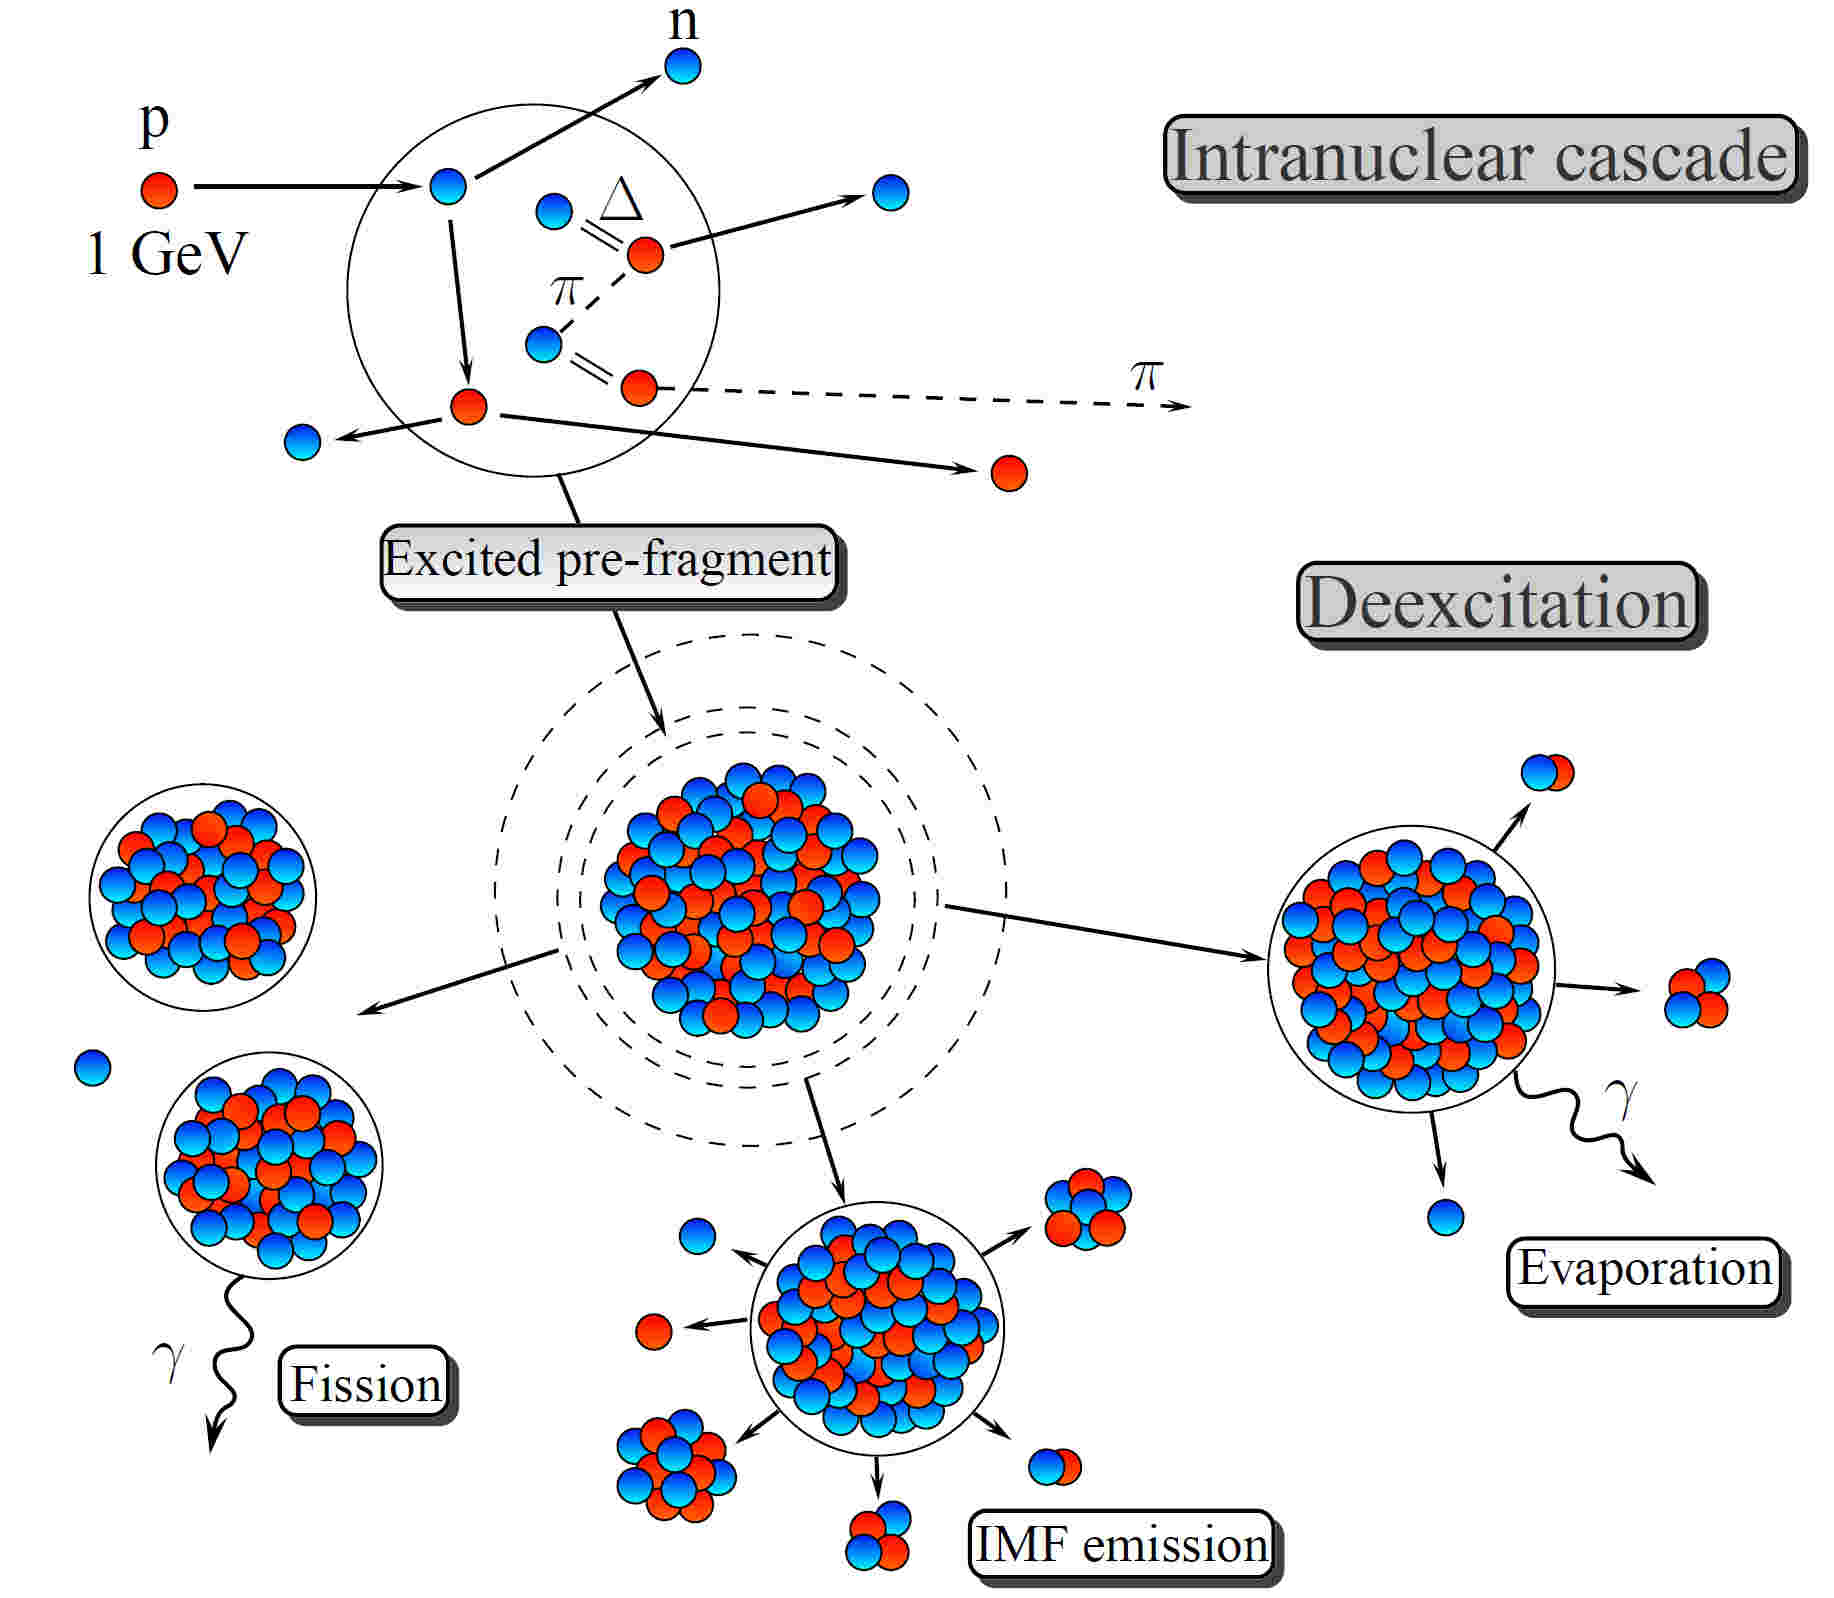
\includegraphics[width=\textwidth]{01_Introduction/figures/fig000_spallation}
	\end{center}
	\caption[Schematic view of the spallation process.]{Schematic view of the spallation process \cite{gorbinet:tel-00660583}. The incident proton interact with nucleons of the target nucleus. An intranuclear cascade occurs leaving the target atom at excited state. Depending of property of the excited nucleus different de-excitation process may occur.}
	\label{chap1:fig:spallation}
\end{figure}


  \section{The need of a European Spallation Source}
  \label{ch1:Summary}
  Neutron probe is a popular tool in the European scientific community and for a long time Europe was a leader in neutron production. However, the future does not look so good with a decrease of the time access on neutron lines for scientists. These are the conclusions of an European Strategy Forum on Research Infrastructures (\acrshort{esfri}) report in 2016 \cite{neutron2016}.

  The majority of neutron sources is based on reactors built before the 1980s.
  The LLB reactor is 39 years old whereas ILL reactor diverged in 1967. In Europe, despite the success of ISIS\footnote{ISIS was supposed to operate during 20 years but is still running after 35 years.}, no second generation of pulsed neutron source like SNS has been built. At the same time, only few new reactors have been built in recent years. Most neutron sources will be shut down within less than 20 years.

  The European Spallation Source (ESS) is a project of a new facility delivering an intense pulsed neutron source. ESS is a crucial project to maintain the level of expertise of neutron users in Europe and to stimulate a renewal in neutron production, both in the form of new research reactors and accelerator-driven sources.

  \begin{figure}[!ht]
	\begin{subfigure}[t]{0.5\textwidth}
		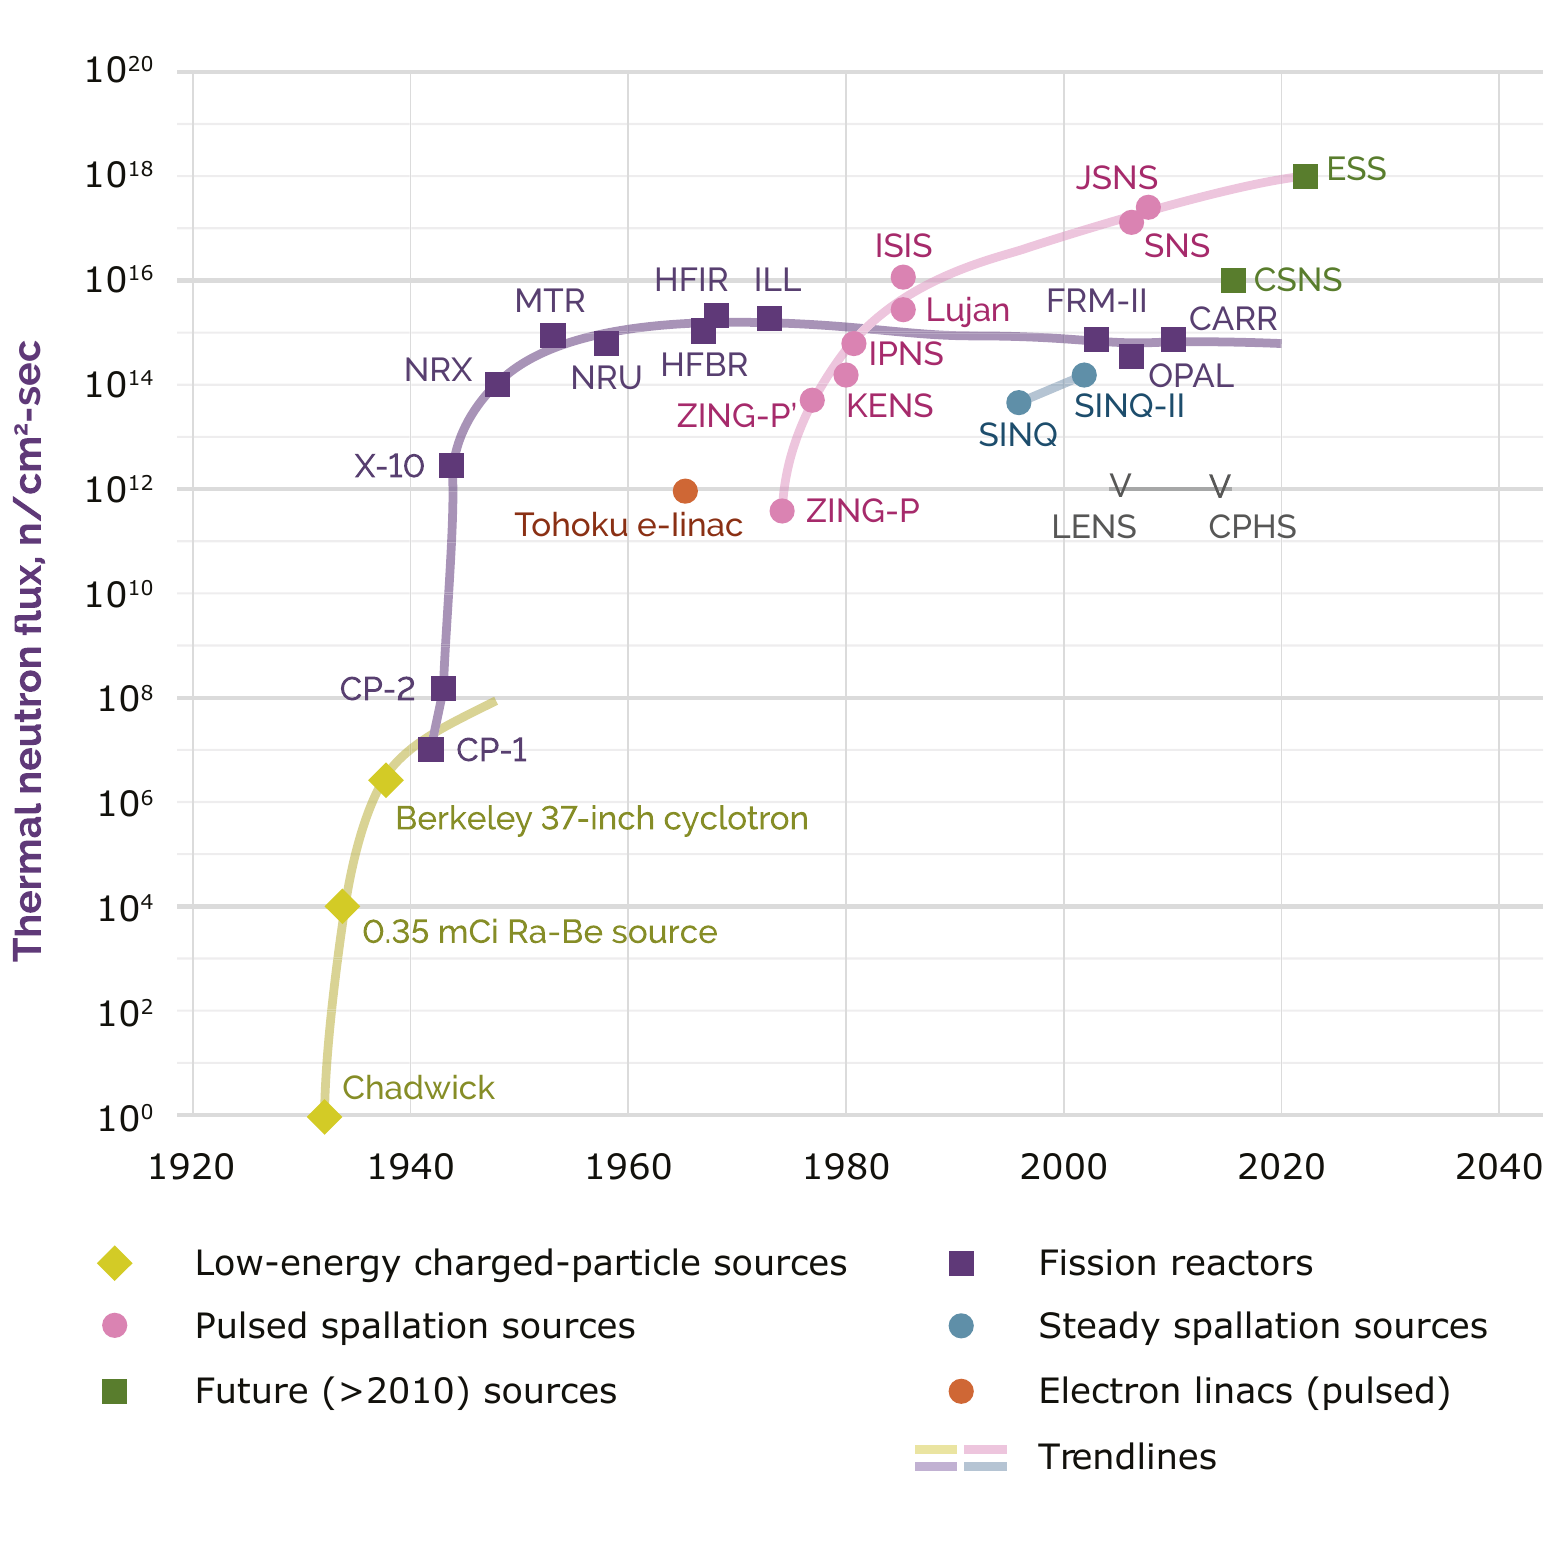
\includegraphics[width=\textwidth]{01_Introduction/figures/fig000_NeutronSources_a}
		\caption{Evolution of thermal neutron sources.}
		\label{}
	\end{subfigure}
	~
	\begin{subfigure}[t]{0.5\textwidth}
		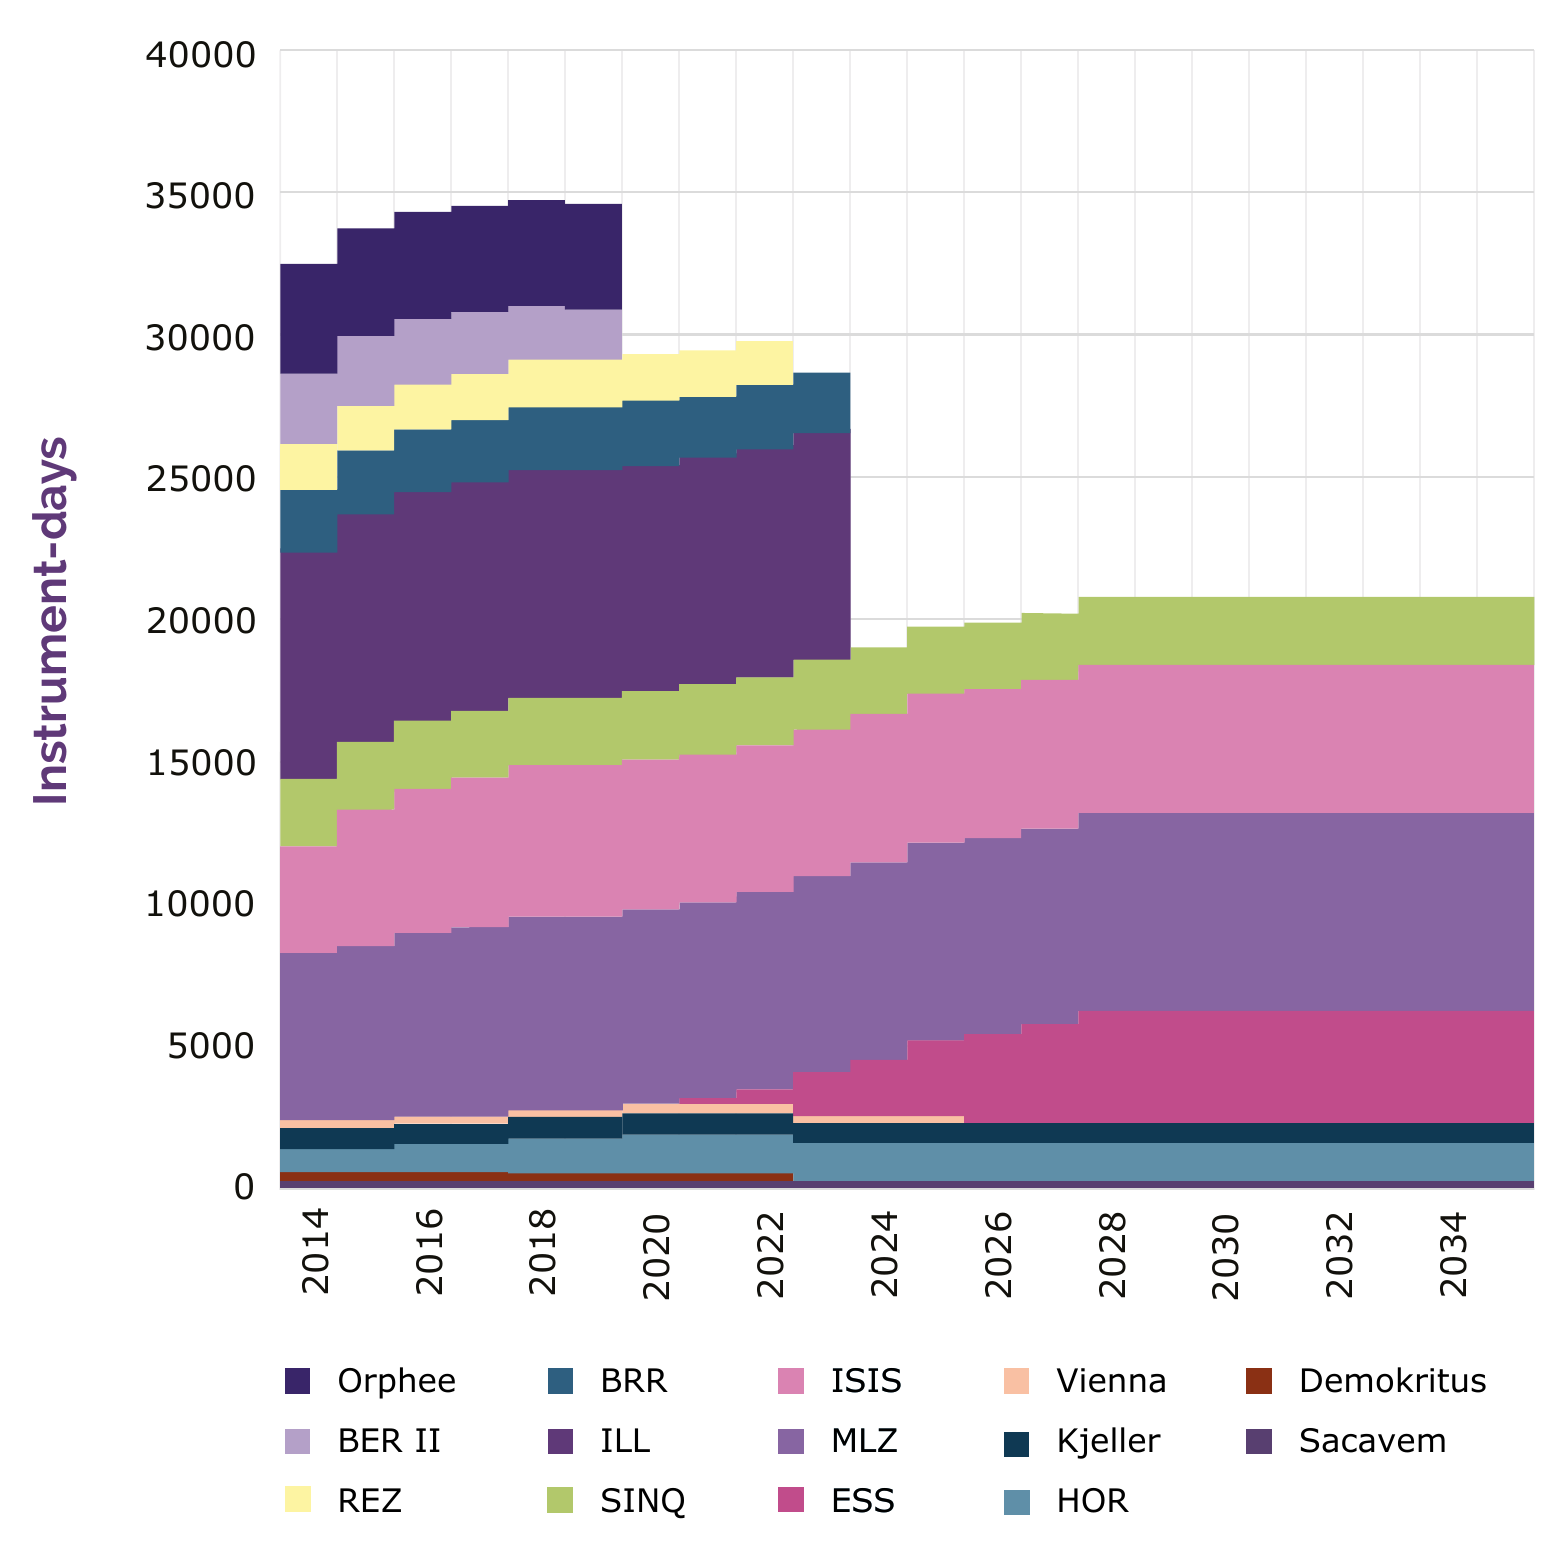
\includegraphics[width=\textwidth]{01_Introduction/figures/fig000_NeutronSources_b}
		\caption{Evolution of beam time for user considering }
		\label{}
	\end{subfigure}
	\caption[]{}
	\label{chap1:fig:NeutronSources}
\end{figure}


  \cleardoublepage
  \section{Bibliography}

  \printbibliography[heading=subbibliography]
\end{refsection}
